\documentclass[11pt]{article}

\usepackage[margin=1in]{geometry}
\usepackage{booktabs}
\usepackage{longtable}
\usepackage{amsmath}
\usepackage{graphicx}
\usepackage{hyperref}
\usepackage{pgfplots}
\pgfplotsset{compat=1.18}

\title{Blossom Failure-Boundary Validation: Finality, Throughput, Correctness, Fault Tolerance, and Network Size}
\author{Blossom Protocol Simulation}
\date{May 21, 2026}

\begin{document}
\maketitle

\begin{abstract}
This report validates the current Blossom protocol failure boundaries with
three repeated long-run simulations per scenario. The focus is the five-axis
tradeoff requested for protocol review: finality, throughput, correctness,
fault tolerance, and network size. The headline result is strong for modeled
safety: all 87 chaos/security runs matched their expected result, all passing
runs finished with one canonical epoch hash, and the repeated matrix reported
zero incorrectly lost local blocks. The performance result is more nuanced.
Trusted mode reaches roughly 5x higher modeled TPS than verified mode at the
same one-way latency because it is dispatch-only. Verified mode pays the echo,
verification, proposal, and commit stages. Both architectures still inherit the
same main scaling issue: full data dissemination creates high wire-byte
amplification as network size grows, especially at 64 nodes with quorum size 6.
\end{abstract}

\section{Method}

The repeated validation run was generated by:

\begin{verbatim}
benchmarks/scripts/run-proof-validation-matrix.sh
benchmarks/scripts/analyze-proof-validation.py benchmarks/results/proof_validation_20260521_024828
\end{verbatim}

The raw run directory is:

\begin{verbatim}
benchmarks/results/proof_validation_20260521_024828
\end{verbatim}

The matrix used three repeats, 2,000 epochs per long scenario, six-member
quorum groups, 32-byte transactions, and the same correctness workloads for the
trusted and verified architectures wherever the claim applies to both. The
verified architecture also ran Byzantine-only checks, because trusted mode does
not claim Byzantine security.

\begin{itemize}
  \item Chaos/security rows: 87 total, 87 matched expectation.
  \item Throughput rows: 72 total, 24 aggregate groups.
  \item Repeat count per aggregate group: 3.
  \item Error bars: sample standard deviation and two-sided 95\% confidence
  interval using the Student t critical value for \(n=3\).
  \item Formal threshold harness: Kani, Creusot, Quint, and Apalache completed
  successfully. Verus remained skipped because the installed binary is the
  crates.io placeholder rather than the verifier.
\end{itemize}

The throughput numbers are modeled protocol wire bytes from the simulator's
message/frame accounting. They are not OS, TCP, TLS, NIC, or observer-service
measurements. In production sizing, those transport costs should be added on
top of the protocol wire rate below.

\section{Protocol Stages}

\begin{longtable}{p{0.16\textwidth}p{0.25\textwidth}p{0.25\textwidth}p{0.23\textwidth}}
\caption{Stage-by-stage risk and mitigation coverage.}\\
\toprule
Stage & Primary risk & Mitigation in the protocol model & Evidence in this run \\
\midrule
\endfirsthead
\toprule
Stage & Primary risk & Mitigation in the protocol model & Evidence in this run \\
\midrule
\endhead
Configuration and identity & Unsafe thresholds, Sybil-style reconnects, or stale identity material & Verified path rejects Byzantine population over \(f=\lfloor(n-1)/3\rfloor\), rejects low repair/reconnect quorums, and binds reconnect to the same node identity & Three fail-closed checks each rejected in all repeats; no pass-run identity loss \\
Block formation & Private local block never enters dissemination & Round-skip accounting distinguishes pre-fanout private data from data that has entered the tree & First-fanout skip intentionally dropped 72,000 local blocks per run; this was classified as intentional, not incorrect loss \\
Topology and quorum selection & Mis-sized quorum or unsafe admission threshold & Six-member quorum groups plus full-set supermajority checks for repair/reconnect admission & Low repair and reconnect quorum checks failed closed in all repeats \\
Dispatch/fanout & Data duplication and bandwidth pressure & Every node disseminates its local subset to peers; manifests and repair carry data once it has entered the tree & Correctness held, but 64-node verified wire bytes reached 523.615 MB/epoch, showing the remaining efficiency cost \\
Echo & Trustless messages may be missing, delayed, or duplicated & Verified path waits for quorum evidence and duplicate votes are not counted as new identities & Byzantine churn with duplicate vote copies passed with zero incorrectly lost blocks \\
Verification & Byzantine peers may replay stale or malformed evidence & State proof and admission checks reject stale, replayed, or identity-shifted reconnect evidence & Byzantine churn ran replay, stale proof, and Sybil attempts across three repeats \\
Proposal & Partitioned or delayed views may produce competing branches & Proposal is gated by the verified stage; partitioned reconnects require catch-up and admission before normal participation & Partition reconnect passed in both architectures; verified path averaged 51,340 reconnect attempts per run \\
Commit/finality & Split finality or divergent epoch hashes & Verified mode commits only after the modeled consensus stages; trusted mode commits after dispatch by assumption & All passing runs ended with one final epoch hash and zero final incorrect active nodes \\
Reconciliation/repair & Correct data may be dropped by transient faults & Runtime reconciliation repairs divergent active nodes and treats non-intentional data loss as a failure & Fault-repair verified 36-node runs repaired \(22{,}943.67\pm636.31\) nodes with zero incorrect loss \\
Drop and reconnect & Faulty nodes may be removed forever or rejoin unsafely & Dropped nodes must ping enough peers and pass admission/catch-up checks before rejoining & Churn and partition scenarios reconnected under load while preserving correctness \\
Round skip assist & A node may assist a future round without carrying data from the missing round & Assists may carry prior finalized data forward; skipped private data before first fanout is intentionally excluded & Skip after first fanout repaired 72,000 node-epoch gaps per run with zero incorrect loss \\
Telemetry/observer & Runtime observation may distort the protocol under test & Telemetry is outside the data-plane safety proof; this matrix uses simulator logs and modeled wire accounting & Report treats traffic as protocol data-plane bytes and excludes observer ingestion overhead \\
\bottomrule
\end{longtable}

\section{Correctness and Fault Tolerance}

Across all repeated passing chaos/security runs, the key correctness invariant
was:

\[
incorrectly\_lost\_local\_blocks = 0
\]

The matrix satisfied this invariant in every passing run. The fail-closed rows
are also counted as successful security checks, because their expected outcome
is rejection before any epoch executes.

\begin{table}[h]
\centering
\caption{Repeated correctness and mitigation checks. Values are mean with 95\% CI where useful.}
\resizebox{\textwidth}{!}{%
\begin{tabular}{lrrrrrrr}
\toprule
Scenario & Architecture & Nodes & Passes & Divergent epochs & Repaired nodes & Reconnect attempts & Incorrect loss \\
\midrule
Fault repair & Verified & 36 & 3/3 & \(1957.67\pm9.41\) & \(22943.67\pm636.31\) & 0.00 & 0 \\
Fault repair & Trusted & 36 & 3/3 & \(1964.00\pm18.76\) & \(23432.67\pm410.35\) & 0.00 & 0 \\
Fault repair & Verified & 64 & 3/3 & \(1740.00\pm26.29\) & \(13663.00\pm1314.57\) & 0.00 & 0 \\
Round skip before fanout & Verified & 36 & 3/3 & \(0.00\pm0.00\) & \(0.00\pm0.00\) & 0.00 & 0 \\
Round skip after fanout & Verified & 36 & 3/3 & \(2000.00\pm0.00\) & \(72000.00\pm0.00\) & 0.00 & 0 \\
Byzantine churn & Verified & 36 & 3/3 & \(4.33\pm1.43\) & \(10.00\pm0.00\) & 456.33 & 0 \\
Partition reconnect & Verified & 36 & 3/3 & \(4.00\pm0.00\) & \(10.00\pm0.00\) & 51340.00 & 0 \\
Reject Byzantine over \(f\) & Verified & 36 & 3/3 & Rejected & Rejected & Rejected & 0 \\
Reject low repair quorum & Verified & 36 & 3/3 & Rejected & Rejected & Rejected & 0 \\
Reject low reconnect quorum & Verified & 36 & 3/3 & Rejected & Rejected & Rejected & 0 \\
\bottomrule
\end{tabular}
}
\end{table}

The round-skip distinction is now explicit. Skipping before first fanout drops
unshared private local blocks by design: the run intentionally dropped 72,000
such blocks per 2,000-epoch run. Skipping after first fanout must not drop the
local block by default, because the block has entered the dissemination tree.
The repeated matrix validated that rule: after-first-fanout skips repaired all
72,000 node-epoch gaps per run with zero incorrectly lost blocks.

\section{Finality and Throughput}

The modeled finality throughput is:

\[
TPS = \frac{N \cdot tx_{node}}{T_f}
\]

where \(N\) is validator count, \(tx_{node}\) is transactions per node per
epoch, and \(T_f\) is modeled finality latency in seconds. The modeled per-node
bandwidth requirement at max modeled throughput is:

\[
B_{node} = \frac{W_{total}}{N \cdot T_f}
\]

where \(W_{total}\) is total modeled protocol wire bytes per epoch. Bandwidth
amplification is:

\[
A = \frac{W_{total}}{B_{epoch}}
\]

where \(B_{epoch}\) is the serialized block data created for that epoch.

\begin{figure}[h]
\centering
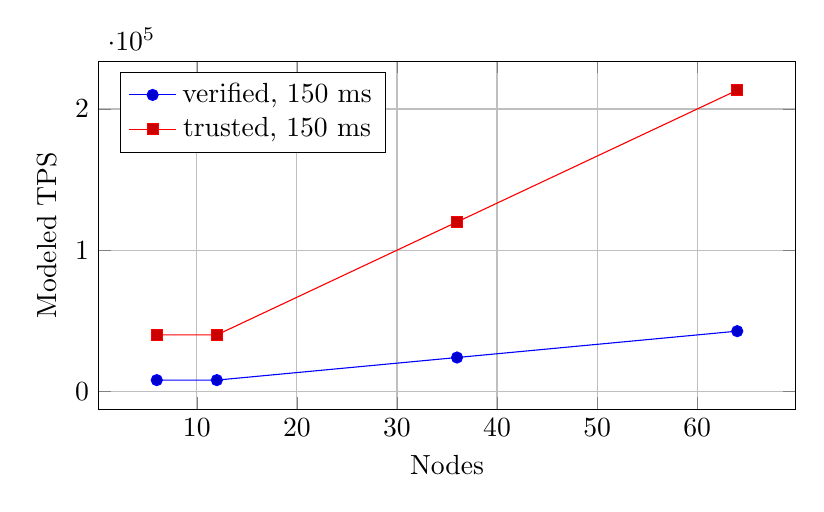
\begin{tikzpicture}
\begin{axis}[width=0.86\textwidth,height=6cm,xlabel={Nodes},ylabel={Modeled TPS},legend pos=north west,grid=both]
\addplot+[mark=*,error bars/.cd,y dir=both,y explicit] coordinates {(6,8000.00) +- (0,0.00) (12,8000.00) +- (0,0.00) (36,24000.00) +- (0,0.00) (64,42666.67) +- (0,0.00)};
\addlegendentry{verified, 150 ms}
\addplot+[mark=square*,error bars/.cd,y dir=both,y explicit] coordinates {(6,40000.00) +- (0,0.00) (12,40000.00) +- (0,0.00) (36,120000.00) +- (0,0.00) (64,213333.33) +- (0,0.00)};
\addlegendentry{trusted, 150 ms}
\end{axis}
\end{tikzpicture}
\caption{TPS by network size at 150 ms one-way latency with 95\% confidence intervals.}
\end{figure}

\begin{figure}[h]
\centering
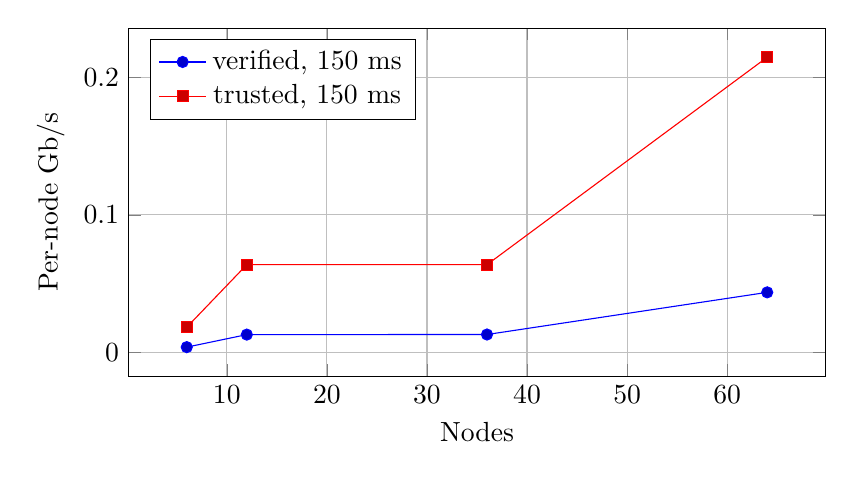
\begin{tikzpicture}
\begin{axis}[width=0.86\textwidth,height=6cm,xlabel={Nodes},ylabel={Per-node Gb/s},legend pos=north west,grid=both]
\addplot+[mark=*,error bars/.cd,y dir=both,y explicit] coordinates {(6,0.003776) +- (0,0.000000) (12,0.012895) +- (0,0.000000) (36,0.012957) +- (0,0.000000) (64,0.043635) +- (0,0.000000)};
\addlegendentry{verified, 150 ms}
\addplot+[mark=square*,error bars/.cd,y dir=both,y explicit] coordinates {(6,0.018264) +- (0,0.000000) (12,0.063782) +- (0,0.000000) (36,0.063782) +- (0,0.000000) (64,0.214728) +- (0,0.000000)};
\addlegendentry{trusted, 150 ms}
\end{axis}
\end{tikzpicture}
\caption{Required per-node protocol traffic capacity at modeled max throughput.}
\end{figure}

\begin{table}[h]
\centering
\caption{Core throughput at 150 ms one-way latency.}
\resizebox{\textwidth}{!}{%
\begin{tabular}{llrrrrrr}
\toprule
Architecture & Nodes & Finality ms & TPS & Total Gb/s & Per-node Gb/s & Wire MB/epoch & Amplification \\
\midrule
Verified & 36 & \(1500.00\pm0.00\) & \(24000.00\pm0.00\) & 0.466439 & 0.012957 & 87.457 & 35.598x \\
Trusted & 36 & \(300.00\pm0.00\) & \(120000.00\pm0.00\) & 2.296138 & 0.063782 & 86.105 & 35.048x \\
Verified & 64 & \(1500.00\pm0.00\) & \(42666.67\pm0.00\) & 2.792615 & 0.043635 & 523.615 & 119.886x \\
Trusted & 64 & \(300.00\pm0.00\) & \(213333.33\pm0.00\) & 13.742580 & 0.214728 & 515.347 & 117.993x \\
\bottomrule
\end{tabular}
}
\end{table}

The trusted path has slightly lower wire bytes per epoch because it does not
send echo, verification, proposal, or commit traffic. It nevertheless shows
higher Gb/s at max modeled throughput because it finalizes five times faster in
the latency model, so it can run five times as many epochs per second. At a
fixed epoch rate, trusted is cheaper; at its own maximum rate, it demands more
network capacity.

\section{Latency Conditions}

The repeated matrix tested even one-way latencies of 50 ms, 150 ms, and 300 ms,
plus random edge latencies from 1 ms to 300 ms. Even-latency rows are
deterministic, so their repeat standard deviations are zero. Random-latency
rows use different latency seeds, so their error bars expose the sensitivity to
the slow supermajority rather than to the arithmetic mean latency.

\begin{figure}[h]
\centering
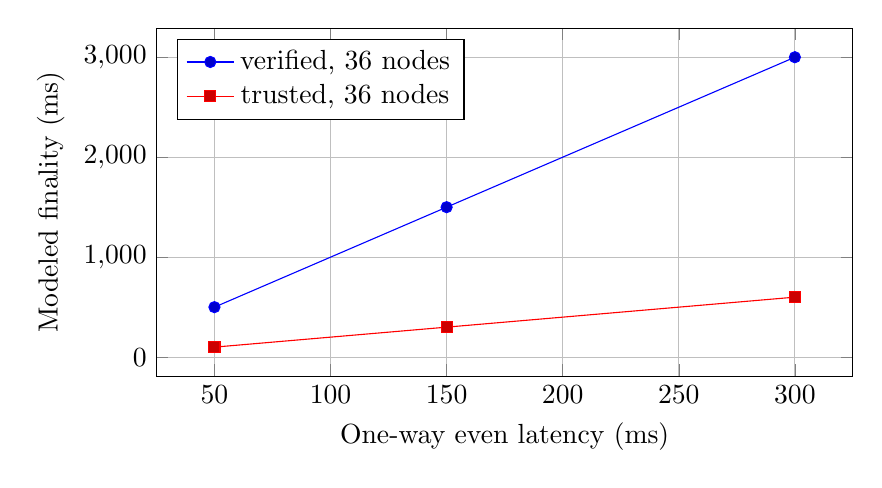
\begin{tikzpicture}
\begin{axis}[width=0.86\textwidth,height=6cm,xlabel={One-way even latency (ms)},ylabel={Modeled finality (ms)},legend pos=north west,grid=both]
\addplot+[mark=*,error bars/.cd,y dir=both,y explicit] coordinates {(50,500.00) +- (0,0.00) (150,1500.00) +- (0,0.00) (300,3000.00) +- (0,0.00)};
\addlegendentry{verified, 36 nodes}
\addplot+[mark=square*,error bars/.cd,y dir=both,y explicit] coordinates {(50,100.00) +- (0,0.00) (150,300.00) +- (0,0.00) (300,600.00) +- (0,0.00)};
\addlegendentry{trusted, 36 nodes}
\end{axis}
\end{tikzpicture}
\caption{Latency sensitivity for the same 36-node workload.}
\end{figure}

\begin{table}[h]
\centering
\caption{Random-latency repeated runs, 1--300 ms per edge.}
\resizebox{\textwidth}{!}{%
\begin{tabular}{llrrrr}
\toprule
Architecture & Nodes & Finality ms & TPS & Per-node Gb/s & Total Gb/s \\
\midrule
Verified & 36 & \(1990.00\pm248.12\) & \(18121.45\pm2301.90\) & \(0.009783\pm0.001243\) & 0.352190 \\
Trusted & 36 & \(412.67\pm76.99\) & \(87581.25\pm17059.94\) & \(0.046551\pm0.009068\) & 1.675822 \\
Verified & 64 & \(2180.00\pm130.87\) & \(29369.27\pm1769.62\) & \(0.030036\pm0.001810\) & 1.922275 \\
Trusted & 64 & \(450.33\pm16.91\) & \(142138.45\pm5301.34\) & \(0.143068\pm0.005336\) & 9.156324 \\
\bottomrule
\end{tabular}
}
\end{table}

The result supports the latency-ceiling model: verified finality is governed by
the slow quorum/supermajority path across five stages, not by average network
latency. Trusted finality is governed by the dispatch path only. This is why the
trusted finality curve is one fifth of the verified curve under even latency.

\section{Real Traffic and Network Requirements}

\begin{table}[h]
\centering
\caption{Required per-node protocol bandwidth for 64 nodes at max modeled TPS.}
\resizebox{\textwidth}{!}{%
\begin{tabular}{llrrrrr}
\toprule
Architecture & Latency profile & Finality ms & TPS & Per-node Gb/s & Total Gb/s & Wire MB/epoch \\
\midrule
Verified & even 50 ms & \(500.00\pm0.00\) & \(128000.00\pm0.00\) & 0.130904 & 8.377846 & 523.615 \\
Trusted & even 50 ms & \(100.00\pm0.00\) & \(640000.00\pm0.00\) & 0.644183 & 41.227741 & 515.347 \\
Verified & even 150 ms & \(1500.00\pm0.00\) & \(42666.67\pm0.00\) & 0.043635 & 2.792615 & 523.615 \\
Trusted & even 150 ms & \(300.00\pm0.00\) & \(213333.33\pm0.00\) & 0.214728 & 13.742580 & 515.347 \\
Verified & even 300 ms & \(3000.00\pm0.00\) & \(21333.33\pm0.00\) & 0.021817 & 1.396308 & 523.615 \\
Trusted & even 300 ms & \(600.00\pm0.00\) & \(106666.67\pm0.00\) & 0.107364 & 6.871290 & 515.347 \\
Verified & random 1--300 ms & \(2180.00\pm130.87\) & \(29369.27\pm1769.62\) & \(0.030036\pm0.001810\) & 1.922275 & 523.615 \\
Trusted & random 1--300 ms & \(450.33\pm16.91\) & \(142138.45\pm5301.34\) & \(0.143068\pm0.005336\) & 9.156324 & 515.347 \\
\bottomrule
\end{tabular}
}
\end{table}

For 64 nodes, the actual epoch payload is 4.368 MB, but the verified protocol
wire total is 523.615 MB/epoch and the trusted wire total is 515.347 MB/epoch.
That is the central efficiency problem in the current design. Most bytes are
dispatch/fanout bytes, not consensus-stage bytes. At 64 nodes the consensus
stages add roughly 8.268 MB/epoch in verified mode, while dispatch alone is
515.347 MB/epoch.

\begin{table}[h]
\centering
\caption{Per-stage protocol traffic at 150 ms one-way latency.}
\resizebox{\textwidth}{!}{%
\begin{tabular}{llrrrrrr}
\toprule
Architecture & Nodes & Dispatch & Echo & Verification & Proposal & Commit & Total wire MB/epoch \\
\midrule
Verified & 36 & 86.105 & 0.430 & 0.306 & 0.563 & 0.052 & 87.457 \\
Trusted & 36 & 86.105 & 0.000 & 0.000 & 0.000 & 0.000 & 86.105 \\
Verified & 64 & 515.347 & 3.056 & 1.734 & 3.294 & 0.184 & 523.615 \\
Trusted & 64 & 515.347 & 0.000 & 0.000 & 0.000 & 0.000 & 515.347 \\
\bottomrule
\end{tabular}
}
\end{table}

This makes the low-hanging performance work clear: optimize dissemination
before optimizing consensus messages. The protocol should move toward
commitment-first dissemination, manifests, repair references, deduplicated
block bodies, dynamic quorum sizing, or a separate data-availability plane.

\section{Network Size}

The 36-node and 64-node results show a sharp topology effect. At 36 nodes,
verified amplification is 35.598x. At 64 nodes, verified amplification is
119.886x. The epoch payload grows from 2.457 MB to 4.368 MB, but wire bytes
grow from 87.457 MB/epoch to 523.615 MB/epoch.

This is not a correctness failure. It is a practical scaling boundary for the
current quorum-size-6 dissemination topology. The tested protocol can preserve
correctness under the modeled faults, but readers should not interpret that as
bandwidth efficiency at arbitrary network size.

\section{Trusted Versus Trustless Interpretation}

Trusted mode represents a permissioned deployment where active nodes are
assumed safe and the protocol can finalize after dispatch. It is useful as an
upper bound on throughput and a lower bound on finality latency. It is not a
Byzantine-secure claim.

Verified mode represents the trustless path. It must pay for echo,
verification, proposal, and commit stages, and it is the only architecture where
Byzantine admission abuse, replay, duplicate votes, stale proofs, and unsafe
thresholds were tested. The repeated runs support the verified safety boundary
within the simulator assumptions:

\[
f = \left\lfloor \frac{n-1}{3} \right\rfloor,\qquad
Q(n)=n-\left\lfloor\frac{n}{3}\right\rfloor
\]

For \(n=36\), the simulator accepted \(f=11\) Byzantine nodes and rejected
\(f+1=12\). It also rejected repair and reconnect quorums below the full-set
supermajority boundary.

\section{Limitations}

These results are strong enough to document the current modeled protocol, but
they are not the last word on production performance.

\begin{itemize}
  \item The traffic numbers are simulator wire bytes, not packet captures from
  a real network stack.
  \item The random-latency model fixes a latency matrix for each 2,000-epoch
  run. A production network study should resample over time windows.
  \item \(n=3\) repeats are enough to expose variance and plot error bars, but
  publication-quality claims should use at least five repeats and broader
  hardware/network diversity.
  \item The protocol remains payload-agnostic. The simulation does not prove
  application-level ledger semantics or smart-contract validity.
  \item Verus is still skipped in the local formal script because the installed
  binary is not the verifier.
\end{itemize}

\section{Conclusion}

The repeated validation supports four practical claims.

\begin{enumerate}
  \item Correctness: the modeled protocol produced zero incorrectly lost local
  blocks across all passing repeated runs.
  \item Fault tolerance: verified mode fails closed at unsafe Byzantine,
  repair-quorum, and reconnect-quorum boundaries.
  \item Finality and throughput: trusted mode is approximately 5x faster in the
  latency model because it skips consensus stages; verified mode pays those
  stages to support trustless operation.
  \item Network size: the dominant production bottleneck is data-plane
  duplication, not consensus-stage overhead.
\end{enumerate}

The next protocol work should keep the threshold proofs and reconciliation
checks intact while reducing repeated full-block transfer. That is the path that
improves throughput and bandwidth without weakening the safety boundary that
the simulator and formal harness just validated.

\end{document}
